При столкновении $\gamma$-квантов с электронами внутренних атомных оболочек
может происходить поглощение квантов. Энергия $\gamma$-кванта передается
соответствующему электрону, а импульс делится между этим электроном и оставшимся
после его вылета ионом. Свободный электрон не может поглотить $\gamma$-квант,
так как при этом невозможно одновременно удовлетворить законам сохранения
энергии и импульса. Наружные электроны не принимают участия в фотоэлектрическом
поглощении, потому что они слабо связаны в атоме, так что их практически можно
считать свободными. Вероятность $dP_{\text{ф}}$ фотоэлектрического поглощения
$\gamma$-квантов пропорциональна длине пути $dl$ и плотности электронов в
среде (в расчет должны приниматься только электроны, принадлежащие внутренним
оболочкам атомов):

\begin{equation}\label{mu ph}
dP_{\text{ф}} = \sigma_{\text{ф}} n_1 dl, \quad \mu_{\text{ф}} = \sigma_{\text{ф}} n_1
\end{equation}

Здесь $ n_1 $ --- плотность внутренних электронов, а $\sigma_{\text{ф}}$ --- поперечное
сечение фотоэлектрического поглощения. Поперечное сечение характеризует
вероятность фотоэффекта, рассчитанную на один электрон. Связь между $\mu_{\text{ф}}$ и
$ \sigma_{\text{ф}} $ устанавливается из формулы \eqref{I(mu)} и в явном виде определяет
зависимости $ \mu $ от плотности среды.

Пусть в результате фотоэффекта энергия $\gamma$-кванта передается электрону,
находящемуся на $ i $-й оболочке атома. Обозначим через $ W_i $ энергию связи
этого электрона. После вылета из атома электрон приобретает кинетическую энергию
$ T_i = \hbar \omega - W_i $. Освободившееся после вылета электрона место
заполняется затем одним из электронов с вышележащих оболочек. При таких
переходах возникает характеристическое рентгеновское излучение.

\begin{wrapfigure}[13]{l}{0.4\linewidth}
  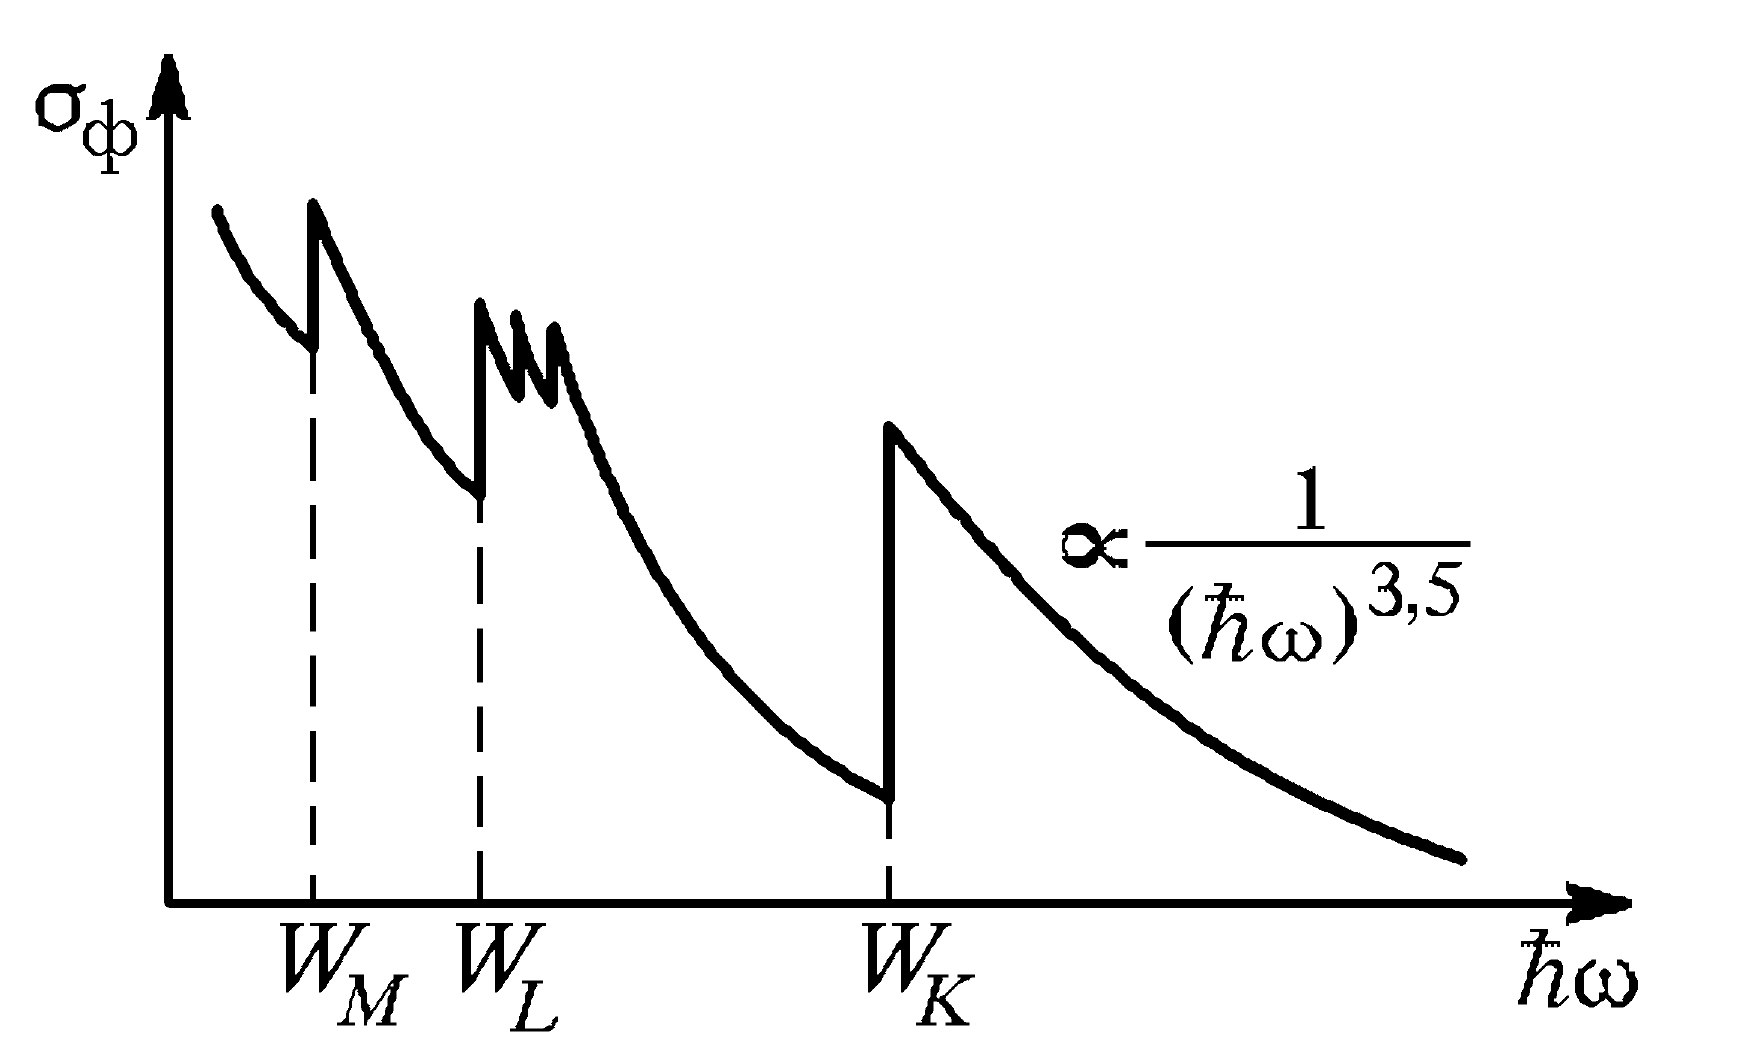
\includegraphics[width=\linewidth]{photo}
  \caption{Зависимость сечения фотоэффекта от энергии $\gamma$-квантов}
  \label{ris photo}
\end{wrapfigure}

Вероятность фотоэффекта сложным образом зависит от энергии $\gamma$-лучей и от
заряда ядер. Для оценок можно пользоваться формулой

\begin{equation}\label{sigma ph}
\sigma_{\text{ф}} \propto \dfrac{Z^5}{(\hbar\omega)^{3,5}}
\end{equation}

Из формулы \eqref{sigma ph} видно, что вероятность фотоэффекта быстро возрастает
при переходе от легких элементов к тяжелым резко падает с увеличением энергии
$\gamma$-квантов. На рис. \ref{ris photo} показана энергетическая зависимость
сечения фотоэффекта. Из рисунка видно, что при энергиях $\gamma$-квантов,
лежащих в области атомных энергий связи, сечение претерпевает резкие изменения:
при возрастании энергии это сечение скачкообразно возрастает, когда становится
возможным выбивание электронов с очередной оболочки (на рис. \ref{ris photo} это
скачки при энергиях $ W_M, W_L, W_K, $ соответствующих энергиям связи $ M, L $
и $ K $-электронов). В этой области сечение фотоэффекта очень велико по
сравнению с сечениями других процессов. Поэтому фотоэффект является доминирующим
механизмом поглощения $\gamma$-квантов при не очень высоких энергиях.
